\trilingualchapter{Concept and Planning: Laying the Foundation}{概念与规划:奠定基础}{Konzept und Planung: Das Fundament legen}{}

The journey of Sue and Owen's restaurant begins with a vision—a concept that will define every aspect of their future establishment. This chapter explores the critical first steps in developing a restaurant concept and creating a comprehensive business plan.

\trilingualsection{The Birth of an Idea}{想法的诞生}{Die Geburt einer Idee}{}

Sue and Owen spent countless evenings discussing their dream restaurant. Sue envisioned a place where traditional techniques meet modern innovation, where every dish tells a story. Owen saw an opportunity to create a sustainable, community-focused establishment that would become a neighborhood cornerstone.

Their concept emerged: \textit{``Artisan Bistro''}—a restaurant that celebrates local ingredients, traditional cooking methods, and warm, welcoming service. This concept would guide every decision they would make.

\trilingualsection{Defining Your Concept}{定义您的概念}{Ihr Konzept definieren}{}

A restaurant concept is more than just a cuisine type—it is the complete identity of your establishment. Consider these elements:

\trilingualsubsection{Cuision Type and Style}{菜系类型与风格}{Küchentyp und Stil}{}
\begin{itemize}
    \item What type of food will you serve?
    \item What is your culinary philosophy?
    \item How will you differentiate from competitors?
    \item What is your price point?
\end{itemize}

\trilingualsubsection{Target Market}{目标市场}{Zielmarkt}{}
\begin{itemize}
    \item Who are your ideal customers?
    \item What are their dining preferences and habits?
    \item What is their average spending capacity?
    \item When and how often do they dine out?
\end{itemize}

\trilingualsubsection{Atmosphere and Ambiance}{氛围与情调}{Atmosphäre und Ambiente}{}
\begin{itemize}
    \item What feeling do you want to create?
    \item Formal or casual?
    \item Family-friendly or adults-only?
    \item Quiet and intimate or lively and energetic?
\end{itemize}

\trilingualsection{Market Research}{市场研究}{Marktforschung}{}

Before committing to a concept, thorough market research is essential. Sue and Owen conducted extensive research:

\trilingualsubsection{Competitive Analysis}{竞争分析}{Wettbewerbsanalyse}{}
\begin{itemize}
    \item Identify direct and indirect competitors
    \item Analyze their menus, pricing, and service models
    \item Visit competitors to understand their strengths and weaknesses
    \item Identify gaps in the market
\end{itemize}

\trilingualsubsection{Demographic Analysis}{人口统计分析}{Demografische Analyse}{}
\begin{itemize}
    \item Population density and growth trends
    \item Income levels and spending patterns
    \item Age demographics
    \item Lifestyle and dining preferences
\end{itemize}

\trilingualsubsection{Location Feasibility}{选址可行性}{Standortmachbarkeit}{}
\begin{itemize}
    \item Foot traffic patterns
    \item Parking availability
    \item Proximity to complementary businesses
    \item Accessibility and visibility
\end{itemize}

\trilingualsection{Business Plan Development}{商业计划制定}{Geschäftsplanentwicklung}{}

A comprehensive business plan is crucial for securing funding and guiding your operations. Sue and Owen's business plan included:

\trilingualsubsection{Executive Summary}{执行摘要}{Zusammenfassung}{}
A concise overview of the business concept, market opportunity, and financial projections.

\trilingualsubsection{Company Description}{公司描述}{Unternehmensbeschreibung}{}
\begin{itemize}
    \item Mission statement
    \item Vision and values
    \item Legal structure (LLC, corporation, partnership)
    \item Ownership structure
\end{itemize}

\trilingualsubsection{Market Analysis}{市场分析}{Marktanalyse}{}
\begin{itemize}
    \item Industry overview
    \item Target market description
    \item Competitive analysis
    \item Market trends and opportunities
\end{itemize}

\trilingualsubsection{Organization and Management}{组织与管理}{Organisation und Management}{}
\begin{itemize}
    \item Organizational structure
    \item Key personnel and their roles
    \item Advisory board or consultants
    \item Hiring plan
\end{itemize}

\trilingualsubsection{Menu and Service}{菜单与服务}{Menü und Service}{}
\begin{itemize}
    \item Sample menu with pricing
    \item Service style and standards
    \item Operating hours
    \item Special events and catering capabilities
\end{itemize}

\trilingualsubsection{Marketing Strategy}{营销策略}{Marketingstrategie}{}
\begin{itemize}
    \item Brand identity and positioning
    \item Marketing channels (social media, print, events)
    \item Public relations strategy
    \item Customer retention programs
\end{itemize}

\trilingualsubsection{Financial Projections}{财务预测}{Finanzprognosen}{}
\begin{itemize}
    \item Startup costs breakdown
    \item Operating expense projections
    \item Revenue forecasts (conservative, realistic, optimistic)
    \item Break-even analysis
    \item Cash flow projections (first 3 years)
    \item Funding requirements
\end{itemize}

\trilingualsection{Financial Planning}{财务规划}{Finanzplanung}{}

\trilingualsubsection{Startup Costs}{启动成本}{Startkosten}{}

Sue and Owen identified the following major startup cost categories:

\begin{table}[h]
\centering
\begin{tabular}{lr}
\toprule
\textbf{Category} & \textbf{Estimated Cost} \\
\midrule
Lease deposits and improvements & \$150,000 \\
Kitchen equipment & \$80,000 \\
Furniture and fixtures & \$40,000 \\
Initial inventory & \$15,000 \\
Licenses and permits & \$5,000 \\
Marketing and branding & \$20,000 \\
Working capital (3 months) & \$50,000 \\
Contingency (10\%) & \$36,000 \\
\midrule
\textbf{Total Startup Costs} & \textbf{\$396,000} \\
\bottomrule
\end{tabular}
\caption{Sample Startup Costs Breakdown}
\end{table}

\trilingualsubsection{Operating Expenses}{运营费用}{Betriebskosten}{}

Monthly operating expenses typically include:
\begin{itemize}
    \item Rent or mortgage
    \item Utilities (electricity, gas, water, internet)
    \item Payroll and benefits
    \item Food and beverage costs
    \item Supplies and smallwares
    \item Marketing and advertising
    \item Insurance
    \item Professional services (accounting, legal)
    \item Maintenance and repairs
    \item Loan payments
\end{itemize}

\trilingualsubsection{Revenue Projections}{收入预测}{Umsatzprognosen}{}

Revenue projections should be based on:
\begin{itemize}
    \item Seating capacity
    \item Average check size
    \item Table turnover rate
    \item Days of operation
    \item Seasonal variations
    \item Growth trajectory
\end{itemize}

\trilingualsection{Legal Considerations}{法律考虑}{Rechtliche Überlegungen}{}

Before opening, Sue and Owen addressed several legal requirements:

\trilingualsubsection{Business Structure}{企业结构}{Unternehmensstruktur}{}
\begin{itemize}
    \item Choose appropriate legal entity (LLC, S-Corp, Partnership)
    \item Register business name
    \item Obtain federal tax ID (EIN)
    \item Register for state and local taxes
\end{itemize}

\trilingualsubsection{Licenses and Permits}{许可证与许可}{Lizenzen und Genehmigungen}{}
\begin{itemize}
    \item Business license
    \item Food service permit
    \item Liquor license (if applicable)
    \item Health department permits
    \item Fire department inspection
    \item Signage permits
    \item Music licensing (if playing copyrighted music)
\end{itemize}

\trilingualsubsection{Insurance}{保险}{Versicherung}{}
\begin{itemize}
    \item General liability insurance
    \item Property insurance
    \item Workers' compensation
    \item Liquor liability (if applicable)
    \item Business interruption insurance
\end{itemize}

\trilingualsection{Timeline and Milestones}{时间表与里程碑}{Zeitplan und Meilensteine}{}

Sue and Owen created a detailed timeline:

\begin{figure}[h]
\centering
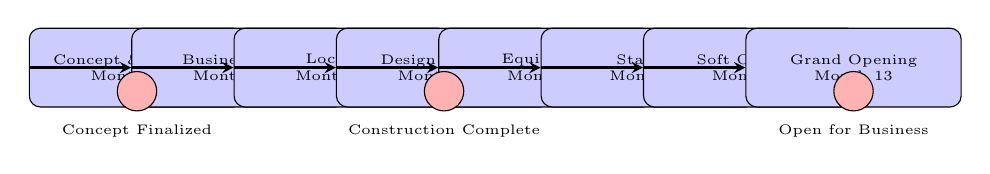
\begin{tikzpicture}[
    node distance=0.8cm,
    auto,
    phase/.style={rectangle, draw, fill=blue!20, text width=2.5cm, text centered, rounded corners, minimum height=1cm, font=\tiny},
    milestone/.style={circle, draw, fill=red!30, minimum size=0.5cm},
    arrow/.style={thick,->,>=stealth}
]
    % Timeline phases
    \node [phase] (p1) {Concept \& Research\\Months 1-2};
    \node [phase, right of=p1, xshift=0.5cm] (p2) {Business Plan\\Months 3-4};
    \node [phase, right of=p2, xshift=0.5cm] (p3) {Location\\Months 5-6};
    \node [phase, right of=p3, xshift=0.5cm] (p4) {Design \& Build\\Months 7-9};
    \node [phase, right of=p4, xshift=0.5cm] (p5) {Equipment\\Month 10};
    \node [phase, right of=p5, xshift=0.5cm] (p6) {Staffing\\Month 11};
    \node [phase, right of=p6, xshift=0.5cm] (p7) {Soft Opening\\Month 12};
    \node [phase, right of=p7, xshift=0.5cm] (p8) {Grand Opening\\Month 13};
    
    % Milestones
    \node [milestone, below of=p1, yshift=0.5cm] (m1) {};
    \node [milestone, below of=p4, yshift=0.5cm] (m2) {};
    \node [milestone, below of=p8, yshift=0.5cm] (m3) {};
    
    % Arrows
    \draw [arrow] (p1) -- (p2);
    \draw [arrow] (p2) -- (p3);
    \draw [arrow] (p3) -- (p4);
    \draw [arrow] (p4) -- (p5);
    \draw [arrow] (p5) -- (p6);
    \draw [arrow] (p6) -- (p7);
    \draw [arrow] (p7) -- (p8);
    
    % Milestone labels
    \node [below of=m1, yshift=0.3cm, font=\tiny] {Concept Finalized};
    \node [below of=m2, yshift=0.3cm, font=\tiny] {Construction Complete};
    \node [below of=m3, yshift=0.3cm, font=\tiny] {Open for Business};
\end{tikzpicture}
\caption{Restaurant Opening Timeline}
\label{fig:opening_timeline}
\end{figure}

\begin{enumerate}
    \item \textbf{Months 1-2}: Concept development and market research
    \item \textbf{Months 3-4}: Business plan completion and funding
    \item \textbf{Months 5-6}: Location search and lease negotiation
    \item \textbf{Months 7-9}: Design and construction
    \item \textbf{Month 10}: Equipment installation and setup
    \item \textbf{Month 11}: Staff hiring and training
    \item \textbf{Month 12}: Soft opening and final preparations
    \item \textbf{Month 13}: Grand opening
\end{enumerate}

\trilingualsection{Key Takeaways}{关键要点}{Wichtige Erkenntnisse}{}

\begin{itemize}
    \item A well-defined concept is the foundation of success
    \item Thorough market research prevents costly mistakes
    \item A comprehensive business plan is essential for funding and operations
    \item Financial planning must be realistic and include contingencies
    \item Legal compliance cannot be overlooked
    \item A detailed timeline keeps the project on track
\end{itemize}

As Sue and Owen completed their planning phase, they felt confident and prepared. The foundation was laid, and they were ready to move forward with finding the perfect location and bringing their vision to life.
